\chapter{QAM信号量子接收机}
在上一章中,我们回顾了现有的一些量子接收机实现方案,
包括二元检测和多元的PSK和PPM检测量子接收机。
但是到目前为止,专门针对QAM信号设计的量子接收机
研究还比较少。然而,QAM信号具有很高的频谱效率,
已被应用到大容量光通信系统之中\cite{winzer2012high}。
因此,研究QAM信号量子接收机是一件很有必要的事情。

\section{QAM信号接收机理论极限}
\subsection{标准量子极限}
在经典通信系统中,常用外差接收机检测QAM信号,
这种接收机的性能也叫QAM信号的标准量子极限(SQL)\cite{kato1999quantum}。
设$M$阶QAM信号由$M$个相干态构成,如图\ref{fig:QAM-signals}所示,
显示的是16-QAM和36-QAM星座图。假设$M$阶QAM信号每一个
正交幅度$X$或$P$都可以取$L$个不同的值,那么$M=L^2, L=3,4,5...$。
设这$L$元基本符号集合为$\Omega = \{-(L-1) + 2(i-1) | i=1,2,...,L\}$,
那么$M$阶QAM信号
可以表示为
\begin{equation}
\begin{split}
\ket{\alpha_{uv}} &= \ket{\alpha(u + j v)}, \\
u, v &\in \Omega.
\end{split}
\end{equation}



\begin{figure}
\centering
  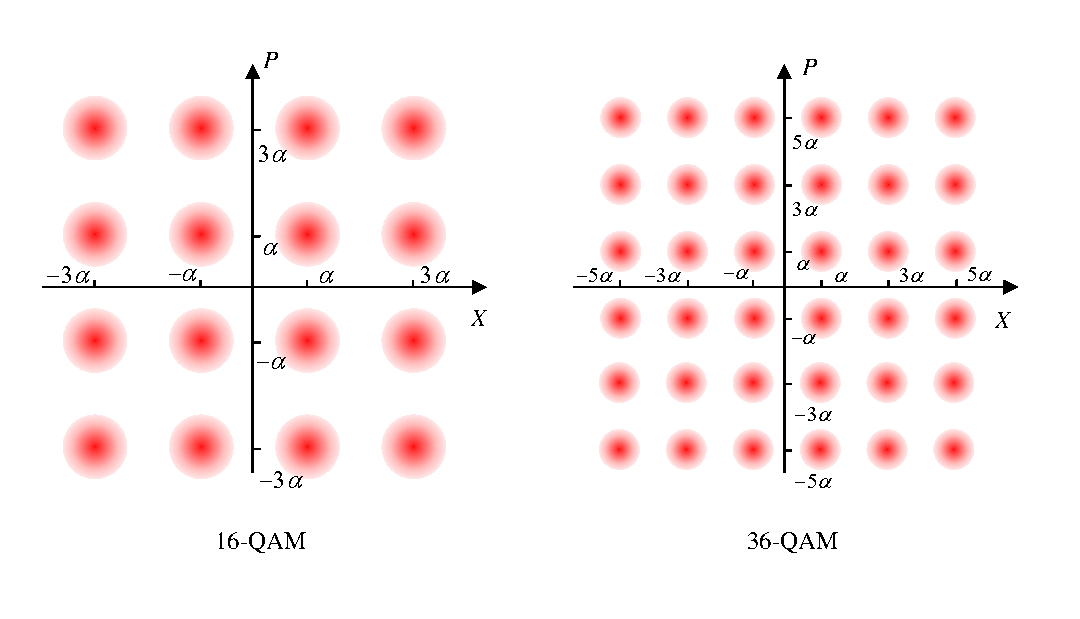
\includegraphics[width=0.8\textwidth]{figures/chap3/QAM-signals}
  \caption{QAM信号星座图}
  \label{fig:QAM-signals}
\end{figure}


利用式\ref{eq:Her-receiver-output}可得理想情况下,
外差接收机的概率密度函数为

的平均错误概率
\subsection{Helstrom极限}


\section{QAM信号Bondurant接收机}


\section{QAM信号自适应分区检测接收机}


\section{QAM信号混合接收机}


\section{三种接收机的对比}

